\cotefile{161-2}
\scanpage{37}
% archive sheet number: 36
\usetikzlibrary{shapes.geometric}

\diagram{\resizebox{\linewidth}{!}{\begin{tikzcd}[ampersand replacement=\&,row sep=small,column sep=small]
\&\text{anneau}\&\&\\
\text{anneau local}\arrow[ur]\&\&\text{anneau réduit}\arrow[ul]\&\text{\shortstack{spectre compact\\(\unsure{séparé})}}\arrow[l]\\
\text{anneau str.\ local}\arrow[u]\&\text{anneau intègre}\arrow[ur]\&\text{pseudocorps}\arrow[u]\arrow[ur]\&\\
\&\text{corps}\arrow[u]\arrow[ur]\arrow[r,dash]\&{}\&{}\arrow[ul,dash]
\end{tikzcd}}}

\[
\widetilde{R}_{\mathrm{zar}}\qquad
\left(A[T]/FA[T]\right)_{\unsure{F'_{*}|F'_{x}|F'}}
\]

\diagram{\begin{tikzcd}[ampersand replacement=\&,row sep=small]
X_i\arrow[d]\& /\& A^{n}\\
Y\&\deleted{\unsure{i}}\arrow[r,dash]\&Y\& U\arrow[ul]\\
\&F\arrow[d]\\
\&G\&{}\arrow[l]
\end{tikzcd}}

\figure{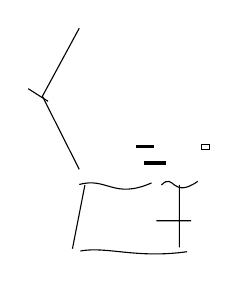
\begin{tikzpicture}[x=.36cm,y=.32cm]
\draw (-3,5.6)--(-4.3,2.9)--(-3,0); \draw (-4.8,3.2)--(-4.1,2.7);
\draw[very thick] (-1,.9)--(-.35,.9) (-.7,.25)--(.05,.25); \draw (1.3,.8) rectangle (1.58,1);
\draw (-3,-.6) .. controls (-2,-.3) and (-1.8,-1.2) .. (-.45,-.54);
\draw (-.1,-.62) .. controls (.36,-.1) and (.25,-1.2) .. (1.18,-.48);
\draw (-2.8,-.62)--(-3.24,-3.15) (.53,-.62)--(.53,-3.1) (-.28,-2.04)--(.95,-2.04) (-2.96,-3.24).. controls (-2,-3.05) and (-1,-3.55)..(.8,-3.27);
\end{tikzpicture}}

% margin note written sideways
\margin{$\forall f(a)\ \exists\unsure{e|\deleted{e}}\in\Pi(M)$ tel que $fe$ inv. et $f(1-e)$ \unsure{nilp.}}

\diagram{\resizebox{\linewidth}{!}{\begin{tikzcd}[ampersand replacement=\&,row sep=small,column sep=small]
\text{str. local}\arrow[dr]\&\&\text{\deleted{loc. intègre}}\arrow[d,dash]\\
\&\text{Spect. connexe}\arrow[d,dash]\&\text{\unsure{loc. irr.|loc. irréd.}}\arrow[d,dash]\\
\&\text{spectre irréd}\arrow[dl,dash]\arrow[dr]\&\text{\deleted{\unsure{loc. réd.}}}\&\text{\uline{réduit}}\arrow[dl]\arrow[dr]\&\&\text{spectre compact}\arrow[dl]\\
{}\&\&\text{\unsure{loc. int}}\arrow[d]\&\&\text{ps. corps}\arrow[ddl,dash]\\
\&\&\text{intègre}\arrow[dl]\&\\
\&\text{intègre normal}\arrow[d]\&\&\text{corps}\arrow[ul,dash]\\
\&\text{régulier dim $\leq$\unsure{1}}\&\&\text{(régulier dim \unsure{0})}
\end{tikzcd}}}

\diagram{\begin{tikzcd}[ampersand replacement=\&]
\Pi\arrow[d]\&[-4pt]{\subset} A\arrow[r,"{p\mapsto p^2-p}"]\& A\\
e\&[-4pt]\text{fini ?}
\end{tikzcd}}

\deleted{\unsure{anneau loc. anneau}}\quad
\deleted{\unsure{produit fini de}}\quad
\unsure{produit fini de connexes}\quad $=$ \unsure{quasi-irréductible}

\diagram{\resizebox{\linewidth}{!}{\begin{tikzcd}[ampersand replacement=\&,row sep=small,column sep=small]
{}\&\text{\uline{connexe}}\arrow[dl]\arrow[dr,dash]\&\&\text{\uline{loc$^{t.}$ irréd}}\arrow[dl]\arrow[dr]\&\&\text{\uline{réduit}}\arrow[dl,dash]\arrow[dr,Rightarrow]\&\&\text{\uline{spectre compact}}\arrow[dl]\\
\text{local}\&\&\text{\uline{irréd}}\&\text{\deleted{\unsure{quasi}}\uline{\unsure{connexe}}}\&\text{\uline{loc$^{t}$ int}}\arrow[dl,dash]\&\deleted{\unsure{corps}}\&\text{\uline{ps.-corps}}\&\\
\text{\deleted{\unsure{str local}} str. local}\arrow[u]\&\&\&\text{\uline{intègre}}\arrow[ul,dash]\&\&\text{\deleted{\unsure{quasi-}}\unsure{quasi-corps}}\arrow[ul,dash]\arrow[ur,dash]\&\\
\text{ultralocal}\arrow[u]\&\&\&\&\text{\shortstack{corps\\\deleted{\unsure{corps sép. clos}}}}\arrow[ul,dash]\arrow[ur,dash]\arrow[uuullll,dash]\\
\&\&\&\&\text{corps \deleted{\unsure{alg.}} sép. clos}\arrow[u,dash]\arrow[uuullll,dash]\&\text{\uline{\unsure{lég.es|lég$_s$}}}\\
\&\&\&\&\text{\shortstack{corps alg clos\\\deleted{\unsure{anneau}}}}\arrow[u,dash]\arrow[uuullll,dash]
\end{tikzcd}}}

\diagram{\begin{tikzcd}[ampersand replacement=\&,column sep=small]
\unsure{e|\varnothing}\arrow[r,"\sim"]\&\Pi(M)\subset A\\
e\arrow[dr,dash]\&(1-e)\arrow[d,dash]\&{}\\
\&\deleted{\unsure{A}}\&\unsure{f=}\arrow[u,dash]\\
\& f^n\& f
\end{tikzcd}}

\[
\begin{aligned}
&\forall f\quad\exists e\ \unsure{\mathrm{id}} \qquad fg=0\qquad g=f^nh\\
&A\xrightarrow{\sim}A_f\times\unsure{A/fA^{*}|A/f^{n}A}
\end{aligned}
\]

$f^n A$ \uline{stationnaire !}\qquad \deleted{$F$}

\[
 V(f)\longrightarrow V(f^n)
\]

\diagram{\begin{tikzcd}[ampersand replacement=\&,row sep=small]
\text{réduit}\arrow[dr]\&\&\text{\shortstack{loc. irréd.\\$=$ qu. irréd.}}\arrow[dl,dash]\arrow[dr,dash]\\
\&\text{\deleted{\unsure{loc.}} intègre}\&\&\text{irréd}
\end{tikzcd}}

localisations ne peut \unsure{subsister|subsérir}\qquad
mais local n'a pas \unsure{néc$^{t}$ d'alg.|d'él$^{ts}$ de} \unsure{nilpotents|nilpotence}
\deleted{\unsure{local$^{t}$ hensélien}}\quad
\uline{\unsure{demande à être|demander à être}}\quad \uline{artinien} \uline{non}

% margin note written sideways
\margin{$D_n\subset\overset{g}{\unsure{A|\mathbb A}}\times\overset{f}{A}\times\overset{e}{\unsure{A|\overline A}}$}

% margin note written sideways
\diagram{\begin{tikzcd}[ampersand replacement=\&,row sep=small]
\&D_n\arrow[d]\arrow[dl,bend right,"\unsure{p}"']\\
\deleted{\unsure{g}}\arrow[r]\&{A\times\Pi}\\
A\arrow[u,leftrightarrow,sloped,"\unsure{i}"]\&
\end{tikzcd}}

% margin note written sideways
\margin{$\unsure{e'},\ e^2=e\quad f^n(1-e)=0,\ g(1-e)=0,\ (f\mid\deleted{\unsure{\theta}}e),\ fg=e$;
\unsure{inv.} et $f^n|U_{1-e}\ \deleted{\unsure{\ne}}0$;
$\left\{\begin{aligned} f^n(1-e)&=0\\ \deleted{\unsure{f}}g(\deleted{\unsure{f}}1-e)&=0\\gf&=e\end{aligned}\right.$}

\diagram{\resizebox{\linewidth}{!}{\begin{tikzcd}[ampersand replacement=\&,row sep=small,column sep=small,cells={nodes={inner sep=1pt}}]
\&\&|[draw,ellipse]|\text{ann}\arrow[dl,dash]\arrow[d]\arrow[dr,dash]\&\&\&|[draw,rectangle]|\text{local \deleted{\unsure{artinien}}}\&\&1\\
\text{car. $p$\unsure{$^{\rm pur}$}}\&\text{\unsure{annelique}}\&\text{quasicomp}\arrow[dl]\arrow[dr,dash]\&\text{\shortstack{\unsure{annulé} par $p$\\\deleted{\unsure{divis}}}}\arrow[r,dash]\&\deleted{\unsure{alg}}\arrow[d,dash]\&\&\&1\\
\&|[draw,ellipse]|\text{connexe}\arrow[d]\arrow[dr,dash]\&\&\text{quasi-irréd}\arrow[dl]\arrow[dr]\&{}\&|[draw,ellipse]|\text{réduit}\arrow[dl]\arrow[dr,dash]\&|[draw,ellipse]|\text{compact}\arrow[d]\arrow[dr,dash]\&4\\
\&|[draw,ellipse]|\text{local}\arrow[d]\&|[draw,ellipse]|\text{irréd}\arrow[dr]\&\&\text{qu. intègre}\arrow[dl]\arrow[dr]\&\text{\unsure{localisé}}\&|[draw,ellipse]|\text{ps. corps}\arrow[dl]\arrow[dr]\&\text{\uline{\unsure{quasi-fini}}}\\
\&\text{\deleted{\unsure{local strict}}}\&\text{\deleted{\unsure{art hens.}}}\&{}\&\text{\unsure{qu. intégral}}\&{}\&{}\&1\\
\&|[draw,ellipse]|\text{str. loc}\arrow[u]\arrow[d]\&\text{\deleted{\unsure{loc hens.}}}\&|[draw,ellipse]|\text{intègre}\arrow[dr,dash]\&\&\text{qu. corps}\arrow[dl]\arrow[dr]\&\text{\unsure{pr.}}\arrow[u,dash]\&3\\
\&|[draw,ellipse]|\text{ultralocal}\arrow[drrr,dash]\&\&\text{\uline{\unsure{intégralement}}}\&|[draw,ellipse]|\text{corps}\arrow[d]\arrow[dr,dash]\&\&|[draw,ellipse]|\text{\shortstack{\unsure{non,}\\\unsure{sauf}\\\unsure{si on}\\\unsure{fixe $n$}}}\&2\\
\&\&\&\&|[draw,ellipse]|\text{corps sép. clos}\arrow[d]\&{}\&\&1\\
\&\&\&\&|[draw,ellipse]|\text{corps alg clos}\&\&\&\underline{1}\\
\&\&\&\&\&\&\&19
\end{tikzcd}}}

\[
\left\{\begin{aligned}
\text{noethériens}&\quad\text{\uline{non}}\\
\text{régulier \unsure{n.-régulier ?}}&\quad\text{\uline{non}}\\
\text{CM ?}&\quad\text{\uline{non}}\\
\text{Gor ?}&\quad\text{\uline{non}}\\
\text{int. complèt$^{e}$ ?}&\quad\text{\uline{non}}
\end{aligned}\right.
\]

\deleted{\unsure{anneau}}\quad\deleted{\unsure{propriété}}\quad
\unsure{f. f.} sur $\mathbb Z$\quad [prés. finie /$k$]

\uuline{corps parfait}\qquad
$\left\{\begin{aligned}&\text{\uline{compact parfait}}\\&=\text{\uline{pseudocorps parfait}}\end{aligned}\right.$

\scanpage{38}
% archive sheet number: 37

\[
\left\{\begin{aligned}&X_\infty\subset e_{\widehat R}\\&\text{crible de }R\end{aligned}\right.
\]

\[
\begin{aligned}
&\deleted{\unsure{X_{\infty}|X_{\infty}^{\rm af}}}\\
&X_\infty(\mathbb Z)=
 \begin{cases}\varnothing&\text{si }Z_\infty\deleted{\unsure{\ne}}=\varnothing\\
 \{e\}&\text{si } Z_\infty\ne\varnothing\end{cases}\\
&\operatorname{Hom}_{\mathrm{Sch.aff}\simeq\widehat R}(Z,\operatorname{Spec}(\mathbb Q))
\end{aligned}
\]

\diagram{\begin{tikzcd}[ampersand replacement=\&]
\&\widehat R\arrow[d,"\mathrm{ex.g.}"]\\
\operatorname{Pro}R\arrow[ur,"\mathrm{ex.g.}"]\& R\arrow[l,"\unsure{\mathrm{ca.g}|\mathrm{ex.g.}}"]
\end{tikzcd}}

\diagram{\begin{tikzcd}[ampersand replacement=\&,column sep=small,row sep=small]
\text{sous-topos \deleted{\unsure{ouvert|ouverts}}\inserted{$B'$} de }\widehat R=B\arrow[d]\\
\text{sous objet $S$ de $e_B$ (foncteur ponctuel sur $R^\circ$)}\arrow[d,leftrightarrow]\\
\text{crible $C_R$ de $R$}\arrow[d,leftrightarrow]\& C_R\arrow[r,hook]\& C\\
\text{crible \deleted{\unsure{$R$|$C$}} $C_B$ de $B$}\arrow[d]\\
\text{\deleted{\unsure{$B$}} sous structure distinguée \inserted{$T'$} de $T=$ $T_B$}
\end{tikzcd}}

\[
 B'\xrightarrow{i}B\qquad ((\forall),\ \unsure{\cap\,\eta})
\]

\[
\begin{aligned}
 B'&=B/S\xrightarrow{\mathrm{can.}}B\\
 &=\widehat C_R \mathrel{\unsure{\widehat{\hookrightarrow}|\xrightarrow{i}}} \deleted{\unsure{B}}B=\widehat R\\
 &=\widetilde C_B\quad+ (C_B\text{ avec topo can})\longrightarrow\widetilde B=\unsure{B}\\
 &=\text{Topos classifiant de }\underline{T'},\quad B_{T'}\longrightarrow
 \deleted{\unsure{B_T|\widetilde B}}\quad\deleted{\unsure{=}}\quad\deleted{\unsure{-}}
\end{aligned}
\]

\[
\begin{aligned}
 S&=i_!(e_{B'})\ \unsure{\longmapsto}\ \text{plus petit sous-objet de $e_B$ tel que }
 \chi_i^*(S)=e_{B'},\\
 &\hspace{2em}\text{i.e. $i^*$ transf\textsuperscript{me} $S\to e_B$ en isomorphisme}\\
 &=\left(x\underset{\operatorname{Ob} R}{\longmapsto}
 \left\{\begin{aligned}&\varnothing\ \text{si }x\notin C_R\\&\{x\}\ \text{si }x\in C_R\end{aligned}\right.\right)\\
 &\deleted{\unsure{=}}=\text{plus grand sous objet de $e_B$ qui est dans }/C_B\\
 &=\text{plus grand sous-objet \unsure{$A\hookrightarrow e_B$} de $e_B$ tel que }
 A|S\in T'(\unsure{\xi|E}/\underline S)
\end{aligned}
\]

\[
\begin{aligned}
 C_R&=\{x\in\operatorname{Ob} R\mid \unsure{x/} \in\operatorname{Im\,ess}(i_!:B'\to B=\widehat R)\}\\
 &=\deleted{\unsure{\{}} C/S\\
 &=R\cap C_B\\
 &=\deleted{\unsure{\{x\in\operatorname{Ob}R\mid}}\ \{A\mid B_{/x}\xrightarrow{\unsure{{}^*f}}
 \unsure{f} \in\mathcal D'(R_{/x})\}\qquad
 \text{lire : }A\mid\widehat R_{/x}\models\unsure{T'|F'}(\widehat R_{/x})
\end{aligned}
\]

% margin note written upside down
\[
\begin{aligned}
 &\varinjlim_{\widehat R}D_n\longrightarrow A\\
 &F(A)\xleftarrow{\sim}\lim\\[-2pt]
 &\hspace{2em}\unsure{\text{$n$-modèle}}\quad
 \text{\unsure{$J$-distingué|$T$ distinguée}}
\end{aligned}
\]

% margin note written upside down
\[
\begin{aligned}
 &\forall x\in S,\quad u\colon C_R\longrightarrow \varnothing,\quad -\ \circ\\
 &\unsure{\mu}\ -\ (q,\deleted{\unsure{f(u)}}\ \exists\unsure{f}\ -\ (p,\unsure{\epsilon}))\qquad y\longrightarrow x\\
 &\text{Ann. discrets }\ \unsure{\longrightarrow}\ \text{Ann. artiniens}\\
 &\unsure{P'}\quad\unsure{\text{Ann top}}\quad \lim\qquad X_i\longrightarrow X
\end{aligned}
\]

% margin note written upside down
\[
 X_{\text{anneauté}}\supset P_1\supset P_2\ \unsure{\supset}\qquad \underbrace{\hspace{1.4cm}}_{?}
 \qquad\text{ann. \unsure{étales}}
\]

% margin note written sideways
\margin{$\begin{aligned}
 C_B&=\operatorname{Im\,ess}\,i_!\\
 &=B/S\\
 &=\widehat C_R\lhook\joinrel\xrightarrow{\widehat{\unsure{j|i}}}\widehat R\\
 &=\{x\in B\mid\unsure{\mathop A\limits^{\leftarrow}|A}|x\in T'(B_{/x})\}\\
 T'&=T_{B'},\ (\xrightarrow{T_i}T_B)\\
 &=T_{B/S}\quad T'(\unsure{\xi|E|\varepsilon})=\{\unsure{\xi|\varepsilon}\xrightarrow{f}B,\ f^*(S)\xrightarrow{\sim}e_{\unsure{\xi|\varepsilon}}\}
 \end{aligned}$}

% margin note written sideways
\margin{$(\unsure{\xi}\mapsto\{f:\unsure{\xi}\to B,\ \text{les $f^*(x)$ ($x\in C_R$) \unsure{sont sur} $e_{\unsure{\xi}}$}\})$
et $\{\unsure{\xi}\overset{f}{\longrightarrow}B\overset{\unsure{g|f}}{\longrightarrow}\unsure{\xi},\ x_i:\unsure{g_i}\text{ et tel que les \unsure{$x_i$} à \unsure{$C_B$} couvrent}\}=$}

\scanpage{39}
% archive sheet number: 38

1) anneau (comm. unifère) \quad $X_{\mathrm{ann}}=\widehat R$\quad
$R=\text{schémas affines de t.f.}/\mathbb Z\simeq(\text{alg de t.f. sur }\mathbb Z)^\circ$

\uline{2)} anneau local \quad $X_{\mathrm{anloc}}=\widetilde R_{\mathrm{zar}}$ \quad zar $=$ topologie de Zariski.
($U\simeq U_f\cup U_{1-f}$, cas universel $U=\mathbb A$, $f$ diagonale)

\uline{4)} anneau str. local \quad $X_{\mathrm{anstrloc}}=\widetilde R_{\mathrm{et}}$ \quad et $=$ topologie étale

(local, et pour tout $U$ et sch rel. étale $U'$ sur $U$ avec $U'\to U$ \inserted{\unsure{de schém. fini|de schém. fin.|et schémas finis}} surj.),
``surjectif'' de schémas, \deleted{\unsure{schéma|isomorphisme}} $U'$ a loc. une section sur $U$;
suffit de cas universel $U=A^n$, $U'=\operatorname{Spec\,rel}(\mathcal O_{\mathbb A^n}[T]/(F))_{F'}$,
$F(\unsure{t|T})=T^n+a_1T^{n-1}+\ldots+a_n$, les $a_i$ les $n$ projections de $A^n$, $F'$ dérivée de $F\ldots$

3) anneau local hensélien \quad $X_{\mathrm{anloc\,hen}}=\widetilde R_{\mathrm{hen}}$ \quad hen $=$ topologie hensélienne,
$X_i\to X$ est couvrant ssi $\forall$ anneau local hensélien $A$, $X_i(A)\to X(A)$ l'est

[Si $X'\to X$ dans $R$ est couvrant \inserted{$B'\leftarrow B$} au sens hens, on veut que
$\underline{\operatorname{Hom}}_{\rm an}(B',A)\to\underline{\operatorname{Hom}}_{\rm an}(B,A)$ soit épi.

\uline{5)} anneau ultralocal \quad $X_{\mathrm{anultloc}}=\widetilde R_{\mathrm{fppf}}$ \quad ?

Si $X'\to X$ \deleted{est}\inserted{dans $R$} couvrant pour fppf,
alors $A(X')\to A(X)$ est épi (il suffit de prendre $X'\to X$ \unsure{qui. fini plat|qui soit fini plat|qu. fini plat} et \unsure{même|en} fini et plat
et même dans les cas universels $U=\mathbb A^n$, $U'=\operatorname{Spec}\deleted{\unsure{A[T]/F}}\mathcal O_{\mathbb A^n}[T]/(F)$, $F$ comme dans \unsure{4}).
\uline{Question} Soit $X'\to X$ dans $R$ \deleted{tel} que $\forall$ anneau ultralocal noetherien $A$,
$X'(A)\to X(A)$ est épi, alors $X'\to X$ est-il couvrant fppf ? Résulterait du lemme : tout anneau local noeth $A$
(\unsure{ess$^t$ de|Rés. de} t.f., sur $\mathbb Z$) admet un hom local dans un anneau ultra-local qui est limite inductive d'algèbres fid. plates de t.f. sur $A$.

6) anneau réduit \quad $X_{\rm red}\simeq\widetilde R_{\deleted{\unsure{\rm top}}\rm red}\simeq\widehat R_{\rm red}$

\[
\begin{aligned}
&\underset{\unsure{\mathcal E}}{\deleted{\unsure{S}}e}
 \xrightarrow[\ ]{\sim\,0_A}\varinjlim_n
 (\underbrace{\operatorname{Ker}(A\xrightarrow{x\mapsto x^n} A)}_{\unsure{\mathrm{I\,Ens}|\mathrm{Im}|I(u)}})\\
&\Updownarrow\\
&\forall\ \deleted{\unsure{f\in}}\ V(f^n)\longrightarrow V(f)\quad \forall f\in A(U)\quad n\in\mathbb N
\end{aligned}
\]

\margin{cas universel}

$\mathrm{topred}$ la top. sur $R$ où $X_i\to Y$ est couvrant ssi $\forall U$ réduit, $X_i(U)\to Y(U)$ l'est,
i.e. s'il existe une section sur $Y_{\rm red}$ \deleted{\unsure{pour}}
$R_{\rm red}$ catégorie des \deleted{\unsure{schémas}} \inserted{objets} de $R$ réduits
(peut être \deleted{aussi} considéré comme catégorie des \inserted{sections de $R$}
\deleted{\unsure{quotients de $R$ par $B\to B_{\rm red}$ de $R$ de but réduit correspondant à un hom}} $\unsure{\leftarrow}\operatorname{Spec}$)

\uline{NB} $X_{\rm red}$ peut être défini par \uline{lim} finies
ce qui se voit sur $X_{\rm red}\simeq\widehat R_{\rm red}$ car $R_{\rm red}$ admettant des $\underset{\leftarrow}{\lim}$ finies

\uline{7)} anneau intègre\quad $X_{\rm int}\simeq\widetilde R_{\mathrm{topint}}$

a)
\diagram{\begin{tikzcd}[ampersand replacement=\&,column sep=small,row sep=small]
 A\amalg A \arrow[r,"u"]\&D\arrow[r,phantom,"\subset"]\arrow[d]\& A\times A\arrow[d,"{(x,y)\mapsto xy}"]\\
 \substack{x\mapsto(x,0)\\y\mapsto(0,y)}\&e\arrow[r,"0"]\arrow[ur,phantom,"\mathrm{cart}"]\& A
\end{tikzcd}}

\[
\begin{aligned}
 &u\ \text{\uline{un épi}}\\
 \text{b)}\qquad&\varnothing_{\unsure{\mathcal E}}\xrightarrow{\sim}\operatorname{Ker}(0_A,1_A:e\rightrightarrows A)
\end{aligned}
\]

% margin note written sideways
\margin{\unsure{a)|c)} $V(fg)=V(f)\vee V(g)$ \ $\forall f,g\in A(U)$,\quad b) $V(1_A)=\varnothing_{\mathcal E}$}

\inserted{\uline{NB} b) assuré par la famille vide couvrant l'objet initial $\varnothing_R$ de $R$, pour top int.}

top int la top. sur $R$ où $X_i\to Y$ est couvrant ssi pour toute comp. irréduct.
$Y_\alpha$ de $Y$ avec str. ind. réduite, il y a section au dessus.
\deleted{\unsure{$R_{\rm int}=$ ss-catégorie des objets intègres de $R$}}

Les objets $F\in\widetilde R_{\mathrm{top\,int}}$ sont les $F\in\widehat R$ tels que $\forall X\in\operatorname{ob}R$,
avec $X_i$, $i\in I$ \unsure{famille|famille des} comp. irréd, \unsure{ses} \deleted{\unsure{trans}}forment sommes finies en produits.
$F(X)\to\prod F(X_i)\rightrightarrows\prod F(X_i\times_X X_j)$ exact.

\scanpage{40}
% archive sheet number: 39

\uline{8)} Anneau \unsure{irreductible|irréductible}

\[
 A_{\rm red}\overset{\rm df}{=}A/\underbrace{\varinjlim_n (I_n}_{\text{nilradical }N}=\operatorname{Ker}(A\xrightarrow{x\mapsto x^n}A))
 \quad\text{est intègre}
\]

i.e.\quad a)
\diagram{\begin{tikzcd}[ampersand replacement=\&]
 A\times N\amalg N\times A\arrow[r,"v"]\& D_N\arrow[r,hook]\arrow[d]\& A\times A\arrow[d,"{(x,y)\mapsto xy}"]\\
 \text{$v$ épi}\&N\arrow[r,hook]\arrow[ur,phantom,"\rm cart"]\& A
\end{tikzcd}}

\[
\begin{aligned}
 \mathrm b)\qquad&V(1_A)\simeq\varnothing_{\mathcal E}\\
 \deleted{\unsure{\mathrm{i.e.}\ \forall f}}\quad\text{i.e.}\quad&
 \left\{\begin{aligned}
 &\forall f,g\in A(U),\quad\varinjlim_n V(f^ng^n)\simeq\varinjlim V(f^n)\vee\varinjlim V(g^n)\\
 &V(1_A)\simeq\varnothing_{\mathcal E}
 \end{aligned}\right.
\end{aligned}
\]

$X_{\rm irr}\simeq\widetilde R_{\mathrm{top\,irr}}$\quad top irred la topologie où une famille
\deleted{$X_i\to$}$X$ est couvrante \uline{ssi} $\forall$ comp. \deleted{sont} irréductible \deleted{$Y$} de $X$,
et \deleted{\unsure{la}}\unsure{ss-schéma} \unsure{induit} $T_i$, l'un des $X_i$ a une section sur $T_{\unsure{i\,\rm red|i|\rm red}}$.

On obtient un exemple d'un sous-topos $X_{\rm irr}$ \deleted{\unsure{non quasi-compact}}\inserted{cohérent} du topos cohérent $X_{\rm ann}$.

\uline{NB} Cette topologie n'est pas quasi-compacte, il y a des recouvrements
(de \deleted{\unsure{schémas}} tout schéma \deleted{\unsure{dont les}}\inserted{ayant une} comp. connexe non \deleted{\unsure{quasi}} irréductible)
qui n'admettent pas de ss-rec$^t$ fini

\uline{NB} Les $F\in\operatorname{Ob}X_{\rm irr}\subset\operatorname{Ob}\widehat R$ transforment sommes finies en produits
\inserted{$\operatorname{Ob}\widetilde R_{\mathrm{top\,irr}}$}

\uline{9)} \uline{Anneau connexe} (i.e. à sp. conn.)\quad $X_{\rm conn}=\widetilde R_{\mathrm{top\,conn}}\simeq\widehat R_{\rm conn}$
($R_{\rm conn}$ ss-cat des sch. aff. conn.)

$\forall f\in A(U)$, $f^2=f\Rightarrow f=1$ ou $f=0$ loc.
Suffit dans cas universel $U=A$;

top. où les familles couvrantes $X_i\to X$ sont celles qui ont une section sur les composantes connexes \inserted{\unsure{c.à.d. ens. d'inclusions|cat. ens. d'inclusions} \unsure{crible|vide} si $X=\varnothing$}.

\diagram{\begin{tikzcd}[ampersand replacement=\&,column sep=small,row sep=small]
 \& A\arrow[r,"{x\mapsto x^2-x}"]\arrow[d]\& A\\
 e\amalg e\arrow[r,"u"]\&\Pi\arrow[r]\& e\arrow[u,"0_A"']\&\text{$u$ épi}\\
 \deleted{\unsure{0,1}}\&\text{(projecteurs)}
\end{tikzcd}}

$\widetilde R_{\rm conn}$ \unsure{c'est} préfaisceaux $R^\circ\to(\mathrm{Ens})$ transformant sommes
\deleted{\unsure{(ensemblistes) en produits}} de deux (donc $n\geq 1$) objets en produits
(\uline{NB} si \unsure{seulement} connexes \deleted{\unsure{conn}} mais \unsure{doit} $\ne\varnothing$
on trouverait les foncteurs \unsure{$F$} qui transforment sommes finies en \unsure{sommes}, \unsure{mais}
\unsure{n'envoyant pas|n'envoyons pas} nécess$^t$ \unsure{d'ensemble|d'ens. vide}. O.K.).

\[
 X_{\mathrm{conn}\ne\varnothing}\simeq\widehat R_{\mathrm{conn}\ne\varnothing}
\]

\uline{10)} Anneau \deleted{\unsure{compact}}\inserted{local de dim 0} \deleted{\unsure{(i.e. à spectre compact)}}

\[
\begin{aligned}
 &\forall f\in A(U),\qquad U_f\amalg_{\unsure{R|B}}\varinjlim V(f^n)\longrightarrow U\quad\text{épi}\\
 &\text{Suffit ds cas universel}\qquad A^*\amalg_{\unsure{R|A}}N_A\deleted{\unsure{\rm loc}}
 \longrightarrow A\quad\text{est épi}\quad
 (N_A:=\varinjlim_n(\operatorname{Ker}(A\xrightarrow{x\mapsto x^n}A))
\end{aligned}
\]

\scanpage{41}
% archive sheet number: 40

% margin note written sideways
\margin{\unsure{commun|commune} 2}

% written upside down
\deleted{\unsure{commune|commun} 2 à 2 est $X_{\varnothing}=$ sous topos ponctuel de $X_{\rm ann}$ correspondant à l'anneau nul, et}

\scanpage{42}
% archive sheet number: 41

\[
 X_{\mathrm{cpct}}\simeq\widetilde R_{\mathrm{top\,cpct}}
\]

cpct est la topologie sur $R$ pour laquelle $X_i\longrightarrow X$ est couv.
ssi pour tt anneau \inserted{local} artinien \deleted{\unsure{local}}
(ou \unsure{artinien|artin.|anneau} de dim 0) \deleted{\unsure{absolument quelconque}} $O$, $X_i(O)\to X(O)$ est épimorphique

encore un topos non cohérent (bien que sous-topos d'un topos cohérent)

\textcircled{\scriptsize\uline{11}} \deleted{\unsure{Pseudo}}pseudo-corps $=$ \deleted{\unsure{compact réduit}}
\inserted{Anneau \inserted{réduit} (local de dim 0)}

\[
 A^*\amalg_{\widehat R} A\xrightarrow{\mathrm{incl},\,0_A}A\quad\text{est épi}
\]

$X_{\mathrm{ps.corps}}\simeq\widetilde R_{\deleted{\unsure{\mathrm{top}}}\mathrm{cons}}$\quad cons, top. sur $R$
où les familles couvrantes sont celles qui ont \deleted{\unsure{une section sur toute fibre}} des sections sur chaque fibre.

$\simeq\widetilde R_{\rm cons}$\quad $R_{\rm cons}$ la catégorie des schémas compacts réduits associés aux schémas de t.f. sur $\mathbb Z$, avec top. de Zariski.

$\widetilde R_{\rm cons}$ formé des foncteurs contravariants qui commutent aux \unsure{sommes|lim} finies

\deleted{\textcircled{\scriptsize 12} corps $=$ compact \deleted{\unsure{intègre}}\inserted{intègre} $=$ ps-corps intègre
$=$ pseudo-corps local \deleted{\unsure{(ou quasi-intègre) ou bien local et réduit ou quasi-intègre}}}

% slanted
\margin{clair}\quad\margin{à prouver}

\deleted{\uline{NB} les ss-topos définis dans 1) à 11) \deleted{\unsure{sont}} ont assez de pts, donc sont définis par leurs points.
Il n'est pas clair qu'il en soit nécessairement ainsi pour les intersections de plusieurs de ces sous topos.
Donc pour vérifier que deux intersections sont égales, \deleted{\unsure{il}}\ ou ont des rel d'inclusion déterminées,
il n'est pas sûr qu'il suffira de le vérifier pour leurs pts, i.e. pour les structures ensemblistes.
-- Sauf si on vérifie à chaque fois que les int. envisagées ont assez de pts !}

\deleted{Vérifier donc que un Anneau \unsure{compact|cpct} \deleted{intègre} A est \deleted{\unsure{intègre}} \inserted{local hens.}
ps corps local A est \unsure{intègre} \inserted{corps alg.} ou cpct intègre,}

\deleted{\unsure{D)|2)} La définition signifie que $A:R\to\mathcal E$ transforme sommes \deleted{familles} couvrantes pour ``top. cpct'' en
\deleted{\unsure{fibrés à sommes finies}}, et qu'il transforme familles couvrantes pour ``top. cpct'' en familles couvrantes,
Montrons qu'une famille $X_i\to X$ qui \deleted{\unsure{de}} est couvrante pour topo discrète au dessus de tt $x\in X$
(i.e. $X_i(k)\to X(k)$ est épi pour tt corps $k$) \deleted{\unsure{est transformée}} en famille épi.
Réc. sur $\dim X$ assez évidente.}

\scanpage{43}
% archive sheet number: 42

\textcircled{\scriptsize 12} Anneau compact (i.e. à spectre compact)\quad
$X_{\rm cpct}\simeq\widetilde R_{\mathrm{top\,cpct}}$

$\forall U$, $A(U)$ à spectre cpct i.e.
$\forall f\in A(U)$, $\exists(1)\ e\in A(U)$, $e^2=e$, $ef$ inversible dans $eA(U)$,
\deleted{$e$} $(1-e)f$ nilpotent. Suffit de le faire pour $f$ universel, $U=A$.
On trouve, si $D_n\subset A\times A\times A$ formé des $g,f,e$ avec $e^2=e$
$f^n(1-e)=0$, $g(1-e)=0$, $fg=e$, \unsure{on voit|on voit se|un mono} induit par \deleted{\unsure{pr}} \unsure{proj$_2$}

\[
 i_n:D_n\hookrightarrow A
\]

et la condition est que les $D_n$ couvrent $A$

Pour la top du $R_{\rm top\,cpct}$, sert donc la condition que, si
$D_n=I_n\amalg_R A^*\lhook\joinrel\xrightarrow{i_n}A$
\inserted{attention, c'est une somme \uline{ds $R$}, pas $\widehat R$}
la famille des $i_n$ soit couvrante.

\margin{topologie non cohérente ! A-t-elle assez de pts ??}\quad ?

\textcircled{\scriptsize 13} \uline{Anneau compact réduit} $=$ \uline{pseudo\deleted{\unsure{cor|corps}}corps}
\quad $X_{\rm cpct}\simeq\widetilde R_{\mathrm{top\,ps\,corps}}\simeq\widehat R_{\rm cons}$

$\forall U$, $A(U)$ est ps. cpct i.e. $\forall f\in A(U)$, $A(U)\xrightarrow{\sim}A_f\times A/fA$, i.e.
$\exists(1)\ e\in A(U)$, $e^2=e$, $ef$ inv., $e(1-f)=0$
i.e. $i_1:D_1\hookrightarrow A$ est un isom

ps. corps est la topologie engendrée par les $X'\to X$ qui ont une section fibre par fibre.
(($X_i\to X$) couvrante ssi $\exists\deleted{\unsure{i|i_0}} X_{i_0}\to X$ ainsi)

$R_{\rm cons}$ comme avant, localisée de $R$ pour les \deleted{topologie} flèches \deleted{\unsure{bijectives|bijections}}
à ext. résiduelles triviales.

$\widehat R_{\rm cons}\subset\widehat R_{\unsure{\rm cons|\rm ét|R|\rm cpct}}$ formé des $R^\circ\to\mathrm{Ens}$ qui transforment les flèches précédentes

\textcircled{\scriptsize 14} Corps sép. clos $=$ corps \inserted{str.} hensélien
\quad $X_{\rm corps\,hens}\simeq\widetilde R_{\mathrm{top\,corps\,sépclos}}$

top. corps hens, topologie où les familles couvrantes sont celles \deleted{\unsure{pour lesquelles}}
$X_i\to X$ qui \deleted{\unsure{sont de fibre séparablement}} ont un pt \deleted{\unsure{rationnel}}
séparable (\unsure{ou fini sép.|ou pure$^t$ sép.|i.e. (fini sép.)}) sur chaque $x\in X$

\[
 \simeq\widetilde{(R_{\rm cons})}_{\rm et}\qquad R_{\rm cons}\text{ comme dans 11), avec top. \uline{étale}.}
\]

\scanpage{44}
% archive sheet number: 43

\textcircled{\scriptsize 15} \uline{Corps alg. clos} $=$ corps ultralocal \quad
$X_{\rm corps\,alg\,clos}\simeq\widetilde R_{\rm top\,corps\,alg\,clos}$

topologie où $X_i\to X$ est couvrante si elle est surjective
$\simeq\widetilde R_{\mathrm{cons\,fppf}}$\quad $R_{\rm cons}$ comme dans 11)
topologie fppf $=$ topologie des familles \deleted{\unsure{contenant uniquement des|contenant une}} familles \deleted{surjectives} finies surjectives.

\textcircled{\scriptsize 16} \uline{Anneau \deleted{\unsure{en}} annulé par $n$} ($\geq1$)

\[
 \text{\textcircled{\scriptsize a}}\qquad
 \begin{aligned}n1_A&=0\\ \text{ou}\qquad V(n1_A)&\lhook\joinrel\xrightarrow[\rm isom]{} e_{\mathcal E}\end{aligned}
\]

\[
 X_{\deleted{n\text{-tors}}\mathbb Z/n\mathbb Z}\simeq\widetilde R_{\mathrm{top}\ n\text{-tors}}
 \simeq \widehat R_{\mathbb Z/n\mathbb Z}
\]

% slanted
\margin{\deleted{\unsure{X est distinct}}\quad Sous-topos ouvert de $X_{\rm ann}=\widehat R$\quad
\uline{N.B} $X_{\unsure{1\text{-tors}|1\text{-tors.}}}=X_\varnothing=$ topos ponctuel}

top $n$-tors topologie où $X_i\to X$ est couvrante ssi un des $V(n1_{X_i})\to V(n1_X)$ \deleted{\unsure{est couvrant}} \inserted{une} section
($X_i\times_{\mathbb Z}\mathbb Z/\deleted{\unsure{1}}n\to X\times_{\mathbb Z}\mathbb Z/n\mathbb Z$)
$R_{\mathbb Z/n\mathbb Z}$ \deleted{\unsure{top. de}}\inserted{sous cat.} ple de $R$ formée des \deleted{\unsure{ens}} $X$ qui sont des $\mathbb Z/n\mathbb Z$-schémas

($R_{\mathbb Z/n\mathbb Z}$ peut être considéré comme une catégorie de fractions de $R$ pour les flèches $f$ telles que $f\otimes_{\mathbb Z}\mathbb Z/n\mathbb Z$ bijections)

\deleted{\unsure{b)}} \uline{Ex} Si $n$ premier, ce sont les ``anneaux de car $p>0$

\deleted{\unsure{a)}} \textcircled{\scriptsize b} anneau où $n$ inversible.

\[
 X_{\mathbb Z[1/n]}\simeq\widetilde R_{\mathrm{top}\,\mathbb Z[1/n]}
 \simeq\widehat R_{\mathbb Z\unsure{(1/n]|[1/n]}}
\]

% slanted
\margin{Sous-topos ouvert}

top $\mathbb Z[1/n]$, top. où $X_i\to X$ est couvrante ssi l'un des
$X_i\otimes_{\mathbb Z}\mathbb Z[1/n]\to\deleted{X}X\otimes_{\mathbb Z}\mathbb Z[1/n]$ a une section

$R_{\mathbb Z[1/n]}$, sous-cat. pleine de $R$ des $\mathbb Z[1/n]$ schémas \inserted{aff.} de t.f.

\deleted{\textcircled{\scriptsize c} Soit plus généralement $S\to e_{\widehat R}$ un mono dans $\mathrm{Pro}\,R$, $R=\text{Sch-aff}$ \inserted{$\mathbb Z\to\Lambda$ (épi d'ann)}
d'où $R_{/S}\hookrightarrow R$ sous-catégorie pleine de $R$ (corresp. aux \deleted{\unsure{annx}} anneaux de t.f. sur $\mathbb Z$ qui sont des $\Lambda$-algèbres).}

\deleted{Considérons les Anneaux du Topos $\mathcal E$ qui sont $\Lambda$-algèbres.
(La structure de $\Lambda$ algèbre est elle unique ? Oui, car $\Lambda$ est commençons par le procédé \unsure{standart|standard} au cas ensembliste).
les $\Lambda$-algèbres de $\mathcal E$ sont les fonct. \unsure{foncteurs|ponctuels} $\mathcal E\to\deleted{\rm Ens}(\Lambda\text{-alg.}\leftrightarrow\mathrm{Ann})$
qui sont représentables ensemblistement. Or \deleted{\unsure{il existe}}
\deleted{\unsure{($\Lambda$-alg) $\simeq\operatorname{Hom}$}} On identifiera (Ann) à $\operatorname{Hom}$ (\unsure{$R$, Ens})\unsure{$^{\rm opp}$}}

\scanpage{45}
% archive sheet number: 44

(où $\unsure{C'|\,'}$ signifie exact à g) et $\Lambda$-alg. à
$\underline{\operatorname{Hom}}'(R_\Lambda,\mathrm{Ens})$ où $R_\Lambda$ cat. des schémas de t.f. sur $\Lambda$, le foncteur d'inclusion

\diagram{\resizebox{\linewidth}{!}{\begin{tikzcd}[ampersand replacement=\&,column sep=small,row sep=small]
 \&\underline{\operatorname{Hom}}'(R_\Lambda,\mathrm{Ens})\arrow[r,hook]\&
 \underline{\operatorname{Hom}}'(R,\mathrm{Ens},\,)\\
 {A\mapsto(B\mapsto\operatorname{Hom}_{\Lambda}(B,A))}\&
 (\Lambda\text{-alg})\arrow[u,"\sim"]\&
 (\mathrm{Ann})\arrow[u,"\sim"]\arrow[l,hook]\&
 {A\mapsto(B\mapsto\operatorname{Hom}_{\mathbb Z}(B,A))}\\
 \Lambda\text{-alg}\&\&\mathbb Z\text{-alg}\&\shortstack{$\mathbb Z$-alg.\\$\parallel$\\$\operatorname{Hom}_\Lambda(B_\Lambda,A)$}
\end{tikzcd}}}

est transposé du foncteur $R\longrightarrow R_\Lambda$, $X\to X\otimes_{\unsure{e|\mathbb Z}}\Lambda$ i.e.
$X\mapsto X\times_e S=X\times S$. \inserted{si $A$ un $\Lambda$-alg.}
(qui est en effet exact à g). Donc

\[
 X_{\Lambda\text{-alg}}\simeq\widetilde R_{\Lambda\mathrm{top}}\simeq\widehat R_\Lambda
\]

$\Lambda$-top : $X_i\to X$ couvrante ssi les $X_i\deleted{\unsure{\otimes|\times}}\times_e S\to X\times_e S$ ont une section.
\uline{NB} $R_\Lambda$ est aussi déduit de $R$ par cat. des fractions, en inversant les $f$ telles que $f\times_e S$ un isom.

\[
\begin{aligned}
 \text{\uline{Ex}}\quad &X_{\mathbb Z/n\mathbb Z\text{-alg}},\quad X_{\mathrm{car}\ p}\quad
 (\text{cas particulier}),\quad X_{\mathbb Z[1/n]}\\
 &X_{\mathbb Q}=X_{\mathrm{car.}\,0}=\deleted{\unsure{\mathrm{car}\neq p}}\bigcap_{n\geq2}X_{\mathbb Z[1/n]}
\end{aligned}
\]

\uline{NB} Ce qu'on vient de voir se généralise au cas d'une $R$ quelconque avec $\varprojlim$ finies, et l'espèce de structure correspondante : $T$.
On se donne $\Lambda\in T(\mathrm{Ens})\simeq\operatorname{Ind}R^\circ$, i.e. $S\in\operatorname{Pro} R$,
on suppose que $S\to e_R$ \deleted{\unsure{un}} mono, et on considère $R_S=$ catégorie des fractions de $R$ par les flèches qui deviennent des isom par $\times_e S$,
donc sous-catégorie image ess. de $\operatorname{Pro}R_{/S}$ par $R\to\operatorname{Pro}R_{/S}$, $X\mapsto X\times_e S$. \deleted{\unsure{par}}.
Comme $\operatorname{Pro} R\hookrightarrow\widehat R$, \deleted{\unsure{on peut}} on peut supposer plus gén. $S\in\operatorname{Ob}\widehat R$, \inserted{$S\subset e_{\widehat R}$}
pas néc. dans l'image essentielle de $\operatorname{Pro} R$, et s'intéresser aux $f:\mathcal E\to\widehat R$ tels que
$f^*(\deleted{\unsure{A}}S)\to f^*(e_{\widehat R})=e_{\mathcal E}$ se factorise par $f^*(S)\hookleftarrow e$.
C'est la forme générale des ss-structures qui sont représentées par des \uline{ouverts} du topos classifiant $\widehat R$.

% slanted
\margin{$T(\mathrm{Ens})^\circ$ \inserted{exact à g.}\quad montrer que si $S\in\operatorname{Pro}R$, \unsure{$\exists$ là,} c'est la condition précédente}

\scanpage{46}
% archive sheet number: 45

\underline{16 (suite)}

Plus gén, pour tout mono $S\xrightarrow{i}e_R$ dans $R$,
\inserted{($\forall$ cat. $R$ stable par $\varprojlim$ finies ens. \unsure{petit|petite}\deleted{\unsure{es}})}
d'où sous-catégorie $R_{/S}$ de $R$, \deleted{et sous-catégorie} considérons
(\deleted{\unsure{Obj|les}} $\mathrm{topos}\ R$-\unsure{$\mathcal E$}) les $R\xrightarrow{\varphi}\mathcal E$ \inserted{ex. à g} tels que $\varphi(i)$ un isom.
i.e. $\forall x\in\operatorname{Ob}\mathcal E$, $\operatorname{Hom}(x,-)\circ\varphi:R\underset{\text{ex. à g.}}{\longrightarrow}(\mathrm{Ens})$ a la $=$ propriété.

Or les foncteurs ex. à g. \deleted{\unsure{sur}} $R\to\mathrm{Ens}$ s'identifient (avec renv. des flèches)
aux éléments de $\operatorname{Pro}R$ (sont pro-représentables), et on prend donc les $\xi\in\operatorname{Pro}R$ tels que
$\operatorname{Hom}_{\operatorname{Pro}R}(\xi,S)\ne\varnothing$, i.e. qui sont sur $S$,
donc ce sont ess. les éléments de $\operatorname{Pro}(R_{/S})$, \deleted{donc} ou encore la sous-cat. pleine de
$\mathcal T=(\operatorname{Pro}(R))^\circ=\operatorname{Ind}(\unsure{\mathcal C|\mathcal G|\mathcal S})$ ($\mathcal C=R^\circ$)
\inserted{des $\xi$} qui \deleted{sont} tels qu'il existe un morphisme $\Lambda\to\xi$, où $\Lambda$ est l'objet de $\mathcal C$ correspondant : $S$.

On a pour les structures envisagées le topos \deleted{\unsure{ouvert}}\inserted{classifiant}
$\widehat R_{/S}$, avec $\widehat R_{/S}\xrightarrow{\widehat i}\widehat R$ déduit de $i:R_{/S}\to R$.

\[
\begin{aligned}
 &\text{On a}\quad i_{\unsure{!|1}}^{\deleted{\unsure{*}}}=\text{inclusion de $R_{/S}$ ds $R$},
 \quad i^*(X)=X\times_e S/S\\
 &i_*(\underset{\text{Objet de $R$ sur $S$}}Y)
 =\{ \underset{\operatorname{Ob}R}{X}\longmapsto\operatorname{Hom}_S(X\times S,Y)=\operatorname{Hom}(X\times S,Y)\},\\
 &\text{ou}\quad i_*(\deleted{\unsure{F|Y}}Y)=\underline{\operatorname{Hom}}(S,Y).
 \quad\inserted{\text{variable}}
\end{aligned}
\]

Considérons maintenant une famille $S_\alpha\lhook\joinrel\xrightarrow{i_\alpha}e_R$ \inserted{filtrante} décroissante
de ss-objets de $e_R$, et soit $T'=\bigcap_\alpha T_{S_\alpha}$ \deleted{\unsure{l'espe}} sous-espèce de structure de $T=T_R=T_{\widehat R}$
définie par les conditions $\varphi(i_\alpha)(=f^*(i_\alpha))$, où $\underline{\underline f}:\mathcal E\to B_T=\widehat R$ est isom pour tt $\alpha$.

\uline{Définie} ainsi par la condition sur les $\operatorname{Hom}(\unsure{X|Z|X_\xi},-)\circ\varphi$, on est ramené à examiner le cas du topos ponctuel $\mathcal E=(\mathrm{Ens})$.
\deleted{\unsure{On doit donc considérer les|Oui}} d'où $\xi=(Y_n)\in\operatorname{Ind}\mathcal C$,
$S=(S_\alpha)\in\operatorname{Pro} R$, $\xi\to e_R=e_{\operatorname{Pro} R}$ est un mono ;
les objets envisagés de \unsure{$\mathcal C^\circ$|$\mathcal S$} sont ceux pour les quels il existe un (unique) morphisme $\xi\to\unsure{O|\sigma|0|\mathcal O}$, donc dans
$\operatorname{Pro}R=\mathcal R$ ce sont ceux $x$ qui se factorisent par un (unique)
$x\longrightarrow S\hookrightarrow e_R=e_{\mathcal R}$.
Mais \deleted{\unsure{quelle|quelles}} est la catégorie ens. petite $R'$ avec \uline{lim} classifiante ?
\deleted{\unsure{Le sous-topos|C'est le topos}}\inserted{pour $\widehat{R'}$ est le} $\bigcap_\alpha B_{/S_\alpha}$.
On a déterminé ces pts, mais quels sont ces pts \unsure{ens} ?

% margin note written sideways
\margin{sauf erreur, ce sont les éléments de l'image essentielle de $R\to\operatorname{Pro}R_{/S}$
définis par chgt de base $X\to X\times_e S$, ou encore les éléments de la catégorie
$\varinjlim R_{/S_\alpha}$. On trouve donc
$\bigcap_\alpha B_{T_\alpha}=\bigcap_\alpha\widehat{R_{/S_\alpha}}=\bigcap_\alpha\widehat R_{/S_\alpha}
=\widehat{\varinjlim_\alpha R_{/S_\alpha}}$, la \inserted{petite} catégorie modulaire avec $\varprojlim$
universelle est $\varinjlim R_{/S_\alpha}$ (qui est une catégorie de fractions de $R$ pour les flèches $i$ telles que $i\times_e S$ un iso.
$\widehat{R_{/S_\alpha}}$, $\widehat R_{/S_\alpha}$ plongés dans $B$ par $i_{\alpha *}$, \unsure{non par|un}
\unsure{$i_{\alpha !}!$|$i_{\alpha !}$ !!}}

\scanpage{47}
% archive sheet number: 46

\textcircled{17} \uline{Anneau parfait de car. $p$} ($p>0$

\[
 p\,1_A=0,\qquad A\xrightarrow{x\mapsto x^p}A\quad\text{isom}
\]

% slanted
\margin{en car. $0$, on convient que parfait signifie réduit ?}

NB\quad parfait $\Longrightarrow$ réduit

\[
 X_{p\text{-perf}}=\widetilde{R_{\unsure{\mathrm{top}|\mathrm{sch}}\,p\text{ perf}}}
 =\widehat{R_{p\text{-perf}}}
\]

$R_{p\text{ perf}}$ catégorie des schémas affines \deleted{\unsure{plats|de}} car. $p$ parfaits qui sont clôtures parfaites de schémas de type fini sur $\mathbb Z/p\mathbb Z$.

top. $p$-perf sur $R$ : $X_i\longrightarrow X$ est couvrante si $\exists i_0$, $(X_{i_0})_p\deleted{\ensuremath{\unsure{\times|\to}}}\to(X)_p$ admet une section après passage à la clôture parfaite de $X_p$

\textcircled{18} \uline{\deleted{\unsure{Anneau de corps|Anneau de car.}} \inserted{compact} parfait de car. $p$} ($>0$).

parfait de car. $p$ $\cap$ pr. corps

\[
\begin{aligned}
 X_{\deleted{\ensuremath{\unsure{\mathrm{pr\,corps}|\mathrm{absol.}}}}\,p\text{-perf}}
 &\simeq \widetilde{R_{\deleted{\ensuremath{\unsure{\mathrm{perf}|\mathrm{pr}}}}\,\mathrm{pr\,corps}\,p\text{-perf}}}.\\
 &\simeq R_{\mathrm{cons}\,p\text{-perf}}
\end{aligned}
\]

top. \unsure{quelq. p. parfaite|quasi p parfaite|cpct p-parfaite} : $X_i\to X$ est couv\textsuperscript{te} ssi $\exists i_0$ t.q. $X_{i_0\,p}\longrightarrow X_p$ a un pt radiciel au dessus de tt pt de $X_p$

$R_{\mathrm{cons}\,p\text{-perf}}=$ catégorie des clôtures parfaites des schémas de car. $p$ dans $R_{\mathrm{cons}}$.

\textcircled{19} \uline{Corps parfait} \deleted{\unsure{$(p>0)$|de $p$}} \inserted{(car $p>0$)}

\[
\begin{aligned}
 X_{\mathrm{corps}\,p\text{-perf}}&\simeq
 \widetilde{R_{\mathrm{top\,corps}\,p\text{-perf}}}\simeq\deleted{\ensuremath{\unsure{R|P}}}\\[-2pt]
 &\hspace{1em}\widetilde{R_{\unsure{\mathrm{cons}_p|\mathrm{cons}/p}\,\deleted{\ensuremath{\mathrm{perf}}}\,\mathrm{Zar}}}
\end{aligned}
\]

$X_i\longrightarrow X$ est couvr\textsuperscript{te} ssi $X_{i\,p}\to X_p$ a des pt radiciels \unsure{pts un|fts un|pts au|sur chaque} par fibre.

\deleted{\textcircled{20} \uline{Anneau à caractéristique}}

\deleted{(Anneau parfait (ou compact parfait, ou corps parfait) de car. $p>0$ non précisé (inclut car $0$)}

\deleted{\unsure{$\Delta$.|$\triangle$.|$A$.} On veut que loc sur $\mathbb Z$ il ait les propriétés envisagées.}

\deleted{Soit $C$ l'ens des nbs qui sont soit premiers, soit $0$ ($0$ mis en cas de car. $0$), \deleted{\unsure{et on|donc|Donc}} soit le symbole $\varnothing$. Alors $\mathcal E$. se décompose can\textsuperscript{ment} en $\mathcal E\simeq\coprod_{c\in C}\mathcal U_c$, avec $\mathcal E$ $\unsure{\Delta|A}\mapsto\left.\vphantom{U}\right|\mathcal U_c$ de car. $p$ si $c\ne\varnothing$, et $c\in C$, \unsure{$\Delta|\mathcal U_\varnothing$|$\Delta\mathcal U_\varnothing$}$=0$. Soient alors $X_{p\deleted{\ensuremath{\mathrm{perf}}}}\subset X_{\mathrm{ann}}$, s-to\unsure{pos|pes} immersions}

\deleted{$X_{\infty\deleted{\ensuremath{\unsure{\mathrm{perf}|\mathrm{cons}}}}}\subset$}

\scanpage{48}
% archive sheet number: 47

\deleted{\unsure{20|sa}} $20)$ \uline{Anneau à car.}

loc. sur $\mathcal E$, $A$ est de car $p>0$ ou de car. $0$, i.e. la famille

\[
\begin{aligned}
 &\deleted{\ensuremath{e_{\mathcal E}\longleftarrow\unsure{\mathop{\mathrm{Sup}}\limits_p|{\bigcup}_p}V(p\,1)}}\\
 &\text{des}\qquad
 \left\{\begin{array}{l}
 \deleted{\ensuremath{\unsure{V|p\in P}}}\ V(p.1_A)\hookrightarrow e_{\mathcal E}\\
 \displaystyle\bigcap_{n\geq 1}(e_{\mathcal E})_{n1_A}\lhook\joinrel\nearrow
 \end{array}\right.
\end{aligned}
\]

est épimorphique (cela fait \margin{\deleted{ou encore} $\mathcal E\longrightarrow\widehat R$ se factorise par le sous-topos $\mathrm{Sup}.$} intervenir une $\varprojlim$ \uline{infinie} \unsure{$\bigvee$|$\exists$}, donc ne donne pas l'existence d'un topos classifiant).

Ou encore $\mathcal E\to\widehat R$ se factorise localement sur $\mathcal E$ par la ``réunion'' $V=\deleted{\ensuremath{X}}_{\mathrm{car}>0}$ des sous-topos ouverts \deleted{\ensuremath{V}} $\widehat{R_{\mathbb Z/p\mathbb Z}}\simeq\widehat R_{\mathrm{Sp}\,\mathbb Z/p\mathbb Z}$, et le sous-topos $W=\widehat{R_{\mathbb Q}}$ (qui n'est pas un sous-topos ouvert) avec mêmes images \deleted{inverses}

\[
 X_{\mathrm{car}.}=\widetilde{R_{\mathrm{top.car}}}
\]

\deleted{\unsure{Or|Et}} \unsure{Or|On|Où} ``top car'' est la borne inférieure des ``top car $p$'' pour tt nb premier $p$, et pour $0$, i.e. la famille $X_i\longrightarrow X$ est couvrante ssi pour \inserted{$\forall p$} \deleted{\unsure{$p$, il|il}} \inserted{$y$ inclus $0$} existe un indice $i(p)$ tel que $(X_{i(p)})_p\longrightarrow (X)_p$ (fibre en $p$) ait une section. C'est

(p.ex. la famille des $(X_p\to X,\ p\ \text{premier ou nul})$ est couvrante, et si $X_{\mathbb Q}\ne\varnothing$, il n'y a pas des familles couvrantes plus \unsure{raffinées|raisonnables|cofinales})

\figure{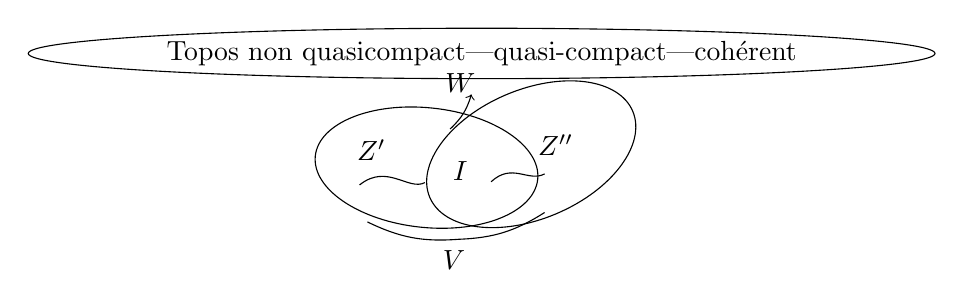
\begin{tikzpicture}[x=1cm,y=1cm]
\node[draw,ellipse,inner sep=2pt] at (2.4,2.3) {Topos non \unsure{quasicompact|quasi-compact|cohérent}};
\draw (1.7,.85) ellipse[x radius=1.42,y radius=.76,rotate=-6];
\draw (3.03,1.02) ellipse[x radius=1.40,y radius=.82,rotate=23];
\draw[->] (2.0,1.34) to[bend right=15] (2.27,1.78);
\node at (2.13,1.93) {$W$}; \node at (1.00,1.07) {$Z'$};
\node at (3.34,1.14) {$Z''$}; \node at (2.13,.81) {$I$};
\draw (.85,.63) .. controls (1.2,.91) and (1.47,.55) .. (1.68,.66);
\draw (2.52,.67) .. controls (2.79,.92) and (2.99,.66) .. (3.20,.77);
\draw (.95,.16) to[bend right=15] (2.11,-.06) to[bend right=15] (3.20,.28);
\node at (2.05,-.33) {$V$};
\end{tikzpicture}}

Plus général\textsuperscript{t}, soit $B$ un topos, $V$ et $W$ deux sous-topos, considérons $T=T_B$ \deleted{\unsure{q|f}} et $T_V$ et $T_W$, enfin $T'=\{\mathcal E\to\{f\colon\mathcal E\to B$, qui se factorise \uline{local\textsuperscript{ment}} par $B$ \uline{ou} $B'$. Cela si\deleted{\unsure{gnifie|gnifie donc}} \unsure{aussi|ainsi}. Cela signifie que : \deleted{l'image} $e_{\mathcal E}=\mathrm{Sup}(e',e'')$, où $e'$ est le plus grand ouvert de $\mathcal E$ \deleted{sur lequel} \inserted{tel que} $f$ t. $\mathcal E_{/e'}$ se factorise par \unsure{$V$|$0$}, et idem pour $e''$. On a alors $f_{B/e'\wedge e''}\longrightarrow V\cap W$, \deleted{et on doit vérifier que} $e'\wedge e''$ est le plus gd ouvert \deleted{\ensuremath{\unsure{A|a}}} $\subset e_{\mathcal E}$ ayant cette propriété ? [si \deleted{si cela} \deleted{\ensuremath{\unsure{B|Z|U}}} est ains\textsuperscript{i}, on a $U\subset e'$, $U\subset e''$, d'où $U\subset e'\wedge e''$, OK.] /

% slanted
\margin{la factoris\textsuperscript{on} d'un \unsure{morphisme|élément} \unsure{par un ss-topos fermé|par ss-topos fermé} ou un ss-topos \unsure{ouvert|un} \unsure{d'une immersion|immersion} !}

S'il y a un topos classifiant pour $T'$, c'est un sous-topos \deleted{\ensuremath{\unsure{A|Z}}} $Z\subset B$ tel que $Z$ \deleted{admet un sous-topos} contenant $V$ et $W$, et ayant des sous-topos ouverts $Z'=Z_{/e'}$, $Z''=Z_{/e''}$, avec $Z'\subset V$, $Z''\subset W$, et \deleted{\ensuremath{\unsure{\mathcal E|Z}}} $\mathrm{Sup}(e',e'')=e_Z$ i.e. $Z=\mathrm{Sup}(Z',Z'')$. (dans l'ens des sous-topos de $Z$, ou de $B$, c'est kif kif). On \unsure{aurait|aurai|aura} donc

\[
 Z=\mathrm{Sup}(Z',Z'')\subset\mathrm{Sup}(V,W)\subset Z
\]

donc $Z=\mathrm{Sup}(V,W)$. De plus on aura \deleted{(ou $Z'$ sera \unsure{l'intersection|l'image} de $Z'$.}

\[
 \begin{aligned}
 \deleted{\text{\unsure{nécessairement|nécessaires}}}\quad
 \deleted{\ensuremath{\unsure{V\times Z|V\times_Z}}}\quad
 Z'&=Z'\cap V'=Z'\times_Z V=\text{ouvert de }V\\
 \unsure{\text{ou }=|\text{ou }-}\qquad Z''&=\text{ouvert de }W
 \end{aligned}
\]

\scanpage{49}
% archive sheet number: 48

(\uline{20 suite})

$Z'\cap Z''$ est un ouvert \deleted{\ensuremath{\unsure{de|Z'}}} de $V\cap W=U$, d'ailleurs $Z$ est obtenu en recollant $Z'$ et $Z''$ suivant $I$ (ouvert commun). De \deleted{\unsure{ce|m|même}} $Z''\cap V$ est un ouvert de $V$, (mais peut-être pas de $Z''$) qui, avec son ouvert $Z'$, recouvre $V$, et $=$ en sens inverse.

% slanted
\margin{Trop compliqué, \unsure{d'abord|donc} établir le calcul de la structure de $T'$, la \unsure{compatib$^{\mathrm{té}}$|complétude} de la fonct\textsuperscript{n} de $e',e''$ aux \unsure{f$^*$|f}, de $f$ à \unsure{base|bas}, \unsure{sans|pour} un raisonn\textsuperscript{t}}

\uline{En résumé} : Pour que le Pb ait une solution, il f et s. \deleted{qu'il existe un ouvert $Z'$ de $V$} que $\exists Z'$ \deleted{est le plus gd} ouvert de $V$ qui induit \deleted{un} ouvert \deleted{sur} $Z'\cap W$ sur $W$, et $Z''$ \deleted{le $2$ plus gd} ouvert de $W$ qui induit un ouvert $Z''\cap V$ sur $V$, alors $V=\mathrm{Sup}(Z',Z''\cap V)$, $W=\mathrm{Sup}(Z'',Z'\cap W)$.

On a vu que c'est nécessaire. Pour voir que c'est suffisant, considérons le topos $\unsure{Z^s|Z|Z^*}$ qui est obtenu en recollant $Z'$ et $Z''$, suivant leur intersection $\unsure{I|Z|Z_1}$, d'où un morphisme $Z\to B$ qui est un plgmt (\uline{à vérifier}) et des morphismes $V\to\unsure{Z^s|Z|Z^*}$ et $W\to Z$ qui sont définis via $Z'\xrightarrow{\mathrm{Id}}Z'$ et $V\cap Z''\longrightarrow Z''$ \deleted{\ensuremath{\unsure{\times_W Z''|\times Z''}}} d'une part ($V=\mathrm{Sup}(Z',V\cap Z'')$) et via \ldots\ d'autre part, qui sont des plgmts (car composés avec $Z\to B$ on obtient les plgmts donnés), donc $V,W\subset Z\subset B$. On voit alors aussitôt que $Z$ satisfait à la condition

% slanted
\margin{construction à préciser}

\uline{NB} Il suffit en particulier que $Z'\cap Z''$ soit ouvert dans $Z'$ et dans $Z''$\ldots.

Dans le cas envisagé $B=\widehat R=X_{\mathrm{ann}}$, $V=X_{\mathrm{car}>0}$, $W=X_{\mathrm{car}\,0}$, on sait que $V$ est déjà un ouvert de $B=\widehat R$ (correspond au crible des objets $X\in\mathrm{Ob}\,R$ qui sont une car positive \deleted{\unsure{fixe|donnée}} \inserted{connue}, \unsure{s.les|sls|savoir}, un premier). NB ce crible \deleted{n'a pas des \unsure{limites produits|produits fibrés}, et} \inserted{a des produits fibrés}, \deleted{\unsure{voyons|mais|noyaux}} mais a des doubles flèches, (mais pas \unsure{des objet|de objet|d'objet} final) et $V\cap W$ est l'ouvert de $X_{\mathrm{car}\,0}\simeq\widehat{R_{\mathbb Q}}$ correspondant à \deleted{l'anneau nul} l'objet nul \inserted{(initial ?)} de $R_{\mathbb Q}$.

Donc \uuline{OK}

\margin{\uline{NB}\quad $X_{\mathrm{car}>0}\simeq\widehat{R_{\mathrm{car}>0}}$, $R_{\mathrm{car}>0}$ sous-cat \unsure{apl.|pl.} de $R$ des schémas ayant une car, $=$ somme amalgamée des $R_{\mathbb Z/p\mathbb Z}$ (\unsure{pr finie|p fini}) sur $\varnothing_R\longrightarrow R_{\mathbb Z/p\mathbb Z}$.}

\scanpage{50}
% archive sheet number: 49

$X_{\unsure{\mathrm{car}{\geq}0|\mathrm{car}}}\simeq\widehat{R_{\mathrm{car}}}$, où $R_{\mathrm{car}}$ est la catégorie somme amalgamée des $\unsure{K_p|R_p}$ (tp fini \deleted{\unsure{sur $\mathbb Z/p$|corps fini}}) sur $\varnothing\longrightarrow R_p$ pour tt $p$, i.e. des schémas \deleted{\unsure{de|sur}} qui sont de type fini sur un corps premier (y inclus $\mathbb Q$) \deleted{\unsure{ayant un|ayant des} \illegible{2}}

21) \uline{Anneaux à car. avec propriétés précisées}

\deleted{\unsure{21)|22)}} \uline{Re NB} On peut repêcher maintenant toutes les notions considérées \inserted{dans le cas de car. donnée en propr\textsuperscript{té} précise} \deleted{ci plus haut, et donner pour} tt $p$ (fini ou infini) un sous-topos \deleted{\ensuremath{\unsure{X|Y}}} $Z(p)$ de $\widehat{R_p}$, on trouvera comme topos modulaire correspondant le topos somme de ceux des $Z(p)$ tels que $\varnothing_p\notin Z(p)$ i.e. l'anneau nul \deleted{\unsure{n'en|n'est}} n'est pas \deleted{dans} du type $Z(p)$, et de la somme amalgamée sur \deleted{la catégorie} \inserted{le topos} ponctuelle des autres $Z(p)$ [munis de leur sous-topos ouvert ponctuel $\varnothing_p$]. Il y a assez de pts ssi chacun des $Z(p)$ \deleted{\unsure{en|on}} a assez

22) Anneau quasi \deleted{\unsure{irrédu|indé}} connexe de rang $\leq n$ (dont le spectre a au plus $n$ comp connexes \deleted{\unsure{$\}$|?}}, donc qui est somme d'au plus $n$ schémas connexes)

\deleted{A} \uline{Déf} On peut trouver loc. une décomposition en produit $A_1\times A_2\times\cdots\times A_n$, avec les $A_i$ connexes $\Longleftrightarrow$ on peut trouver loc. \deleted{d'un produit} des projecteurs $e_i$ ($1\leq i\leq n$) orthogonaux de somme $1$, avec $A_j=A/\sum_{j\ne i}e_j A$ connexe pour tt $1\leq j\leq n$.

\diagram{\begin{tikzcd}[ampersand replacement=\&,row sep=small]
 \Pi_n\subset A^n\arrow[d,hookrightarrow] \\
 e_1,\ldots,e_n\ \text{avec}
\end{tikzcd}}

\[
 \left\{\begin{aligned}
 e_i^2&=e_i\quad\forall i\\
 e_i e_j&=0\quad\forall i,j\quad i\ne j\\
 \sum e_i&=1
 \end{aligned}\right.
\]

\diagram{\begin{tikzcd}[ampersand replacement=\&,row sep=small]
 A\times\Pi_n\arrow[d]\& A_j=A_{\Pi_n}/\displaystyle\sum_{j\ne i}e_j A_{\Pi_n}\arrow[dl]\\
 \deleted{\ensuremath{\unsure{A|p}}}\Pi_n\arrow[d,leftrightarrow]\&\\
 {}\&
\end{tikzcd}}

\diagram{\begin{tikzcd}[ampersand replacement=\&,row sep=small]
 \Pi_n\amalg\Pi_n\arrow[r,"{i_{n,j}}"]\arrow[dr,dash]\&\Pi(A_j)\arrow[d,dash]\quad\text{(proj. de $A_j$)}\\
 \&\Pi_n
\end{tikzcd}}

\unsure{2|?}\qquad soit $\Pi_{nj}\subset R_n$ plus grand ss-objet pour lequel \unsure{$i_{nj}$ un épi.|$i_{nj}$ une épi} commut\textsuperscript{t} avec chgt de base \deleted{dans} \uline{$\mathcal E$}
